\chapter{User Input and Making Plots}\label{chapter:user-input}

\section{Objectives}
In this chapter you are going to see how you can process user input for
changing the parameters of your scan and how to plot the results while
they are being generated. Dealing with user input can lead to unexpected
errors that are sometimes hard to anticipate. Plotting the data while it
is being acquired is a great feature, especially when you want to make
quick decisions before an entire scan is done.

\section{Introduction}
In the previous chapter you have already seen how to handle some user
input: you have a start and a stop button able to trigger the scan. It
is useful, but it doesn't really allow you to change the parameters of
the scan. When you want to take input from a user, you will have to deal
with the validation of the values. More often than not, a user will
mistake the input port with the voltage range, or they will forget what
the \mintinline{python}{delay} does. Sadly, this user can very well be yourself in
the future.

Incorrect input data from a user can not only lead to the wrong
experiment, but it can also mean a big problem in your setup. Imagine that
you set a voltage to a value higher than what your device can handle. Or
you set a piezo stage to a position that will break your sample (a very,
very common issue in microscopes). To avoid these issues, the program
has to check that the input makes sense before being passed to a device,
and this is called data validation.

Having a {GUI} that allows you to change the parameters of an experiment
is very handy. Much more so is to add the possibility to monitor a
signal while the experiment is running. Plotting in real time is not
hard but it can be computationally expensive, depending on how many data
points are you willing to show and how often do you want to update the
plot. In this chapter, you will learn how to develop a program that
takes into account these issues.

If you have experience analyzing data with Python, most likely you have
come across \emph{Matplotlib}, a great library for generating very
professional plots. Even if it is a great tool for making
figures, it is not the proper tool for real-time visualization. Updating
Matplotlib plots is an intensive task for the computer and therefore it
is not going to allow you to update the plots as often as you would
like. That is why, for data visualization, you are going to use another,
perhaps a lesser-known library, called
\href{http://www.pyqtgraph.org/}{PyQtGraph} which integrates everything
that you need for plotting within user interfaces.

\section{Getting User Input}\label{getting-userinput}

\begin{center}
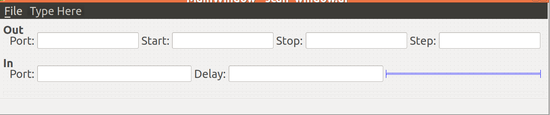
\includegraphics[width=.6\textwidth]{images/scan_window.png}
\end{center}

In your {GUI}, you have added some parameters that the user can modify
before triggering a scan, namely, those are the output port, the start,
stop, and the step of the voltage, the input port, and the delay between
measurements. You need to read the values and update them into the
experiment class before triggering the \mintinline{python}{do_scan} method. If you
remember from the command line example, updating the values of the scan
is as easy as doing
\mint{python}|experiment.properties['Scan']['start'] = new_start|
In the {GUI} it is going to be the same principle. If you want to read
from a \mintinline{python}{QLineEdit} (the name of the widget that holds the
information) you just need to do the following:

\begin{minted}{python}
self.outPortLine.text()
\end{minted}

This command will give us access to whatever is written in the
\mintinline{python}{outPortLine}. Bear in mind that you can not only read from the
line, you can also set the text that you want to display, like this:

\begin{minted}{python}
self.outPortLine.setText("Text to display")
\end{minted}

\exercise{Now that you know how to read and set the values of a
\mintinline{python}{QLineEdit}, update the \mintinline{python}{__init__} method of the
\mintinline{python}{ScanWindow} in order to set the initial values of the scan,
which are available within
\mintinline{python}{experiment.properties['Scan']}.}

To allow the user to change the parameters, you need to read them and
update the experiment class. By now you should have a broad idea on how
to achieve this, but it is important to point out that the experiment
class relies on receiving values with units, not just numbers in the
appropriate parameters. In the chapter when you defined the experiment
class you also impose some restrictions on how the parameters should be
defined. If you go back to the class, you will see that the
\mintinline{python}{do_scan} method transforms strings into quantities. Therefore,
the parameters for the scan should be strings with the appropriate
units, and the experiment class will take care of the conversion.

\begin{minted}{python}
self.experiment.properties['Scan'].update({
        'port_out': int(self.outPortLine.text()),
        'start': self.outStartLine.text(),
        'stop': self.outStopLine.text(),
        'step': self.outStepLine.text(),
        'port_in': int(self.inPortLine.text()),
        'delay': self.inDelayLine.text(),
     })
\end{minted}

Note that you are using a special method of dictionaries called
\mintinline{python}{update}, that allows you to update a dictionary with the values
given by another dictionary. If it is unclear to you how does it work,
you should just practice with an easier example, a dictionary with just
a handful of keys and values. Remember that the experiment class takes
strings for the properties with units, but an integer for the ports,
that is why we transform the input and output ports to \mintinline{python}{int}. It
is as easy as that, few lines of code, little complication and now you
are getting user input into consideration.

When you start playing around with your program, and especially when you
give it to other users to work with, a lot of problems are going to
arise. One of the most common ones is people forgetting to put units
into their values. You can build your entire software just with plain
numbers, but in the long term, this is very unreliable. Soon enough you
will forget if the numbers you were supposed to use were in centimeters,
millimeters, etc. Go ahead and try to see what happens if you don't
include units, or if you try to start the scan when some of the values
are left blank.

Validating user input is a complicated task; at some point, especially
for software that is supposed to be used by smart people with good
intentions, you have just to let it be. For example, you can check that
the output port is a valid option if you have only two outputs it should
be either 1 or 2. But you should also check that the values in every
option are the ones that the device can handle, etc. And then, imagine
they are wrong, what do you do? Do you create a new window with an error
message? It is up to you and your use case to judge how much involvement
is needed.

\exercise{To validate user input, you can also use signals. \mintinline{python}{QLineEdit} has
a signal called \mintinline{python}{editingFinished}, that is triggered whenever you
stop writing and move away from the line. Hook that signal from whatever
input you like to a new method that will verify that the values are
correct (for example, that the output port is either 1 or 2). If the
input is not valid, disable the \mintinline{python}{startButton} by doing
\mintinline{python}{self.startButton.setEnabled(False)}, or the opposite if the
value is correct.}

\section{Plotting the results}\label{plotting-theresults}
Plotting the results while you are acquiring the data is the last step
to have a fully functional program for performing experiments. You may
remember (or you should refresh it if you don't) that the
\mintinline{python}{do_scan} accumulates the data in a variable called
\mintinline{python}{ydata_scan}. It means that each data point is available as soon
as it is acquired. This is true for your very simple daq device, but it
may not be exactly true for more complex acquisition cards. Anyways,
let's see how to plot.

You may remember the PyQtGraph module that you used for plotting some
data while we were looking at running the experiment from within the
command line. You are also going to use it here, and then you are going
to make a plot inside of the \mintinline{python}{ScanWindow}, let's see:

\begin{minted}{python}
import pyqtgraph as pg

[...]

class ScanWindow(QtGui.QMainWindow):
    def __init__(self, experiment, parent=None):
        super().__init__(parent)

        [...]

        self.main_plot = pg.PlotWidget()
        layout = self.centralwidget.layout()
        layout.addWidget(self.main_plot)
        self.ydata = np.zeros(0)
        self.xdata = np.zeros(0)
        self.p = self.main_plot.plot(self.xdata, self.ydata)
\end{minted}

If you remember from a couple of chapters before, when plotting data you
were also defining a \mintinline{python}{PlotWidget}, but at the time you had no
user interface around it. In the previous chapter, you have seen that
the building blocks of Qt are called Widgets, and in the snippet above
you see that everything is coming in place together. The first step is
to create the widget you want to use, in this case, it is called
\mintinline{python}{self.main_plot}. Once you have the widget, you need to add it
to the window. In the previous chapter, you have added buttons to a
\mintinline{python}{ButtonBox}, but the plot should be added to the layout of the
window. At this point is where some explanations regarding Qt are
in order.

When you define windows in Qt Designer, some important things are
happening under the hood. For example, when you define a
\mintinline{python}{QMainWindow}, you should also define the central widget of it,
which is like letting the window know which widget is the most important
one. In the designer, this happens by default and perhaps you don't even
notice that as soon as you create a window, there is also an empty
\mintinline{python}{centralwidget} into which you put all the elements. When you use
Python, you can reference the central widget by
\mintinline{python}{self.centralwidget}. In the \mintinline{python}{ScanWindow} the
\mintinline{python}{centralwidget} has a vertical layout associated with it, and
that you can use by calling the method \mintinline{python}{layout()}. Note that not
all widgets have a default layout defined, sometimes it can even happen
that the layout is a part of the widget, such as any other button,
line, etc.

Once you have access to the layout, you add the plot widget to it.
Because the \mintinline{python}{centralwidget} has a default vertical layout, the
plot will be appended at the bottom. If it would have been a horizontal
layout, it would have been appended to the right, etc. Qt is very
flexible when it comes to specifying where and how widgets look like.
Remember that everything that you have defined in the Designer can be
later changed programmatically. Normally, it is better to have a good
starting point and change the look of your window as little as possible.
After you have added the plot to the layout, you can initialize it with
empty data. In this case, you use two zeros and plot them. If you
remember from a couple of chapters earlier, the output of the
\mintinline{python}{plot} method will allow you to personalize the plot, adding
labels, units or new data. That is why you store it as \mintinline{python}{self.p}.
You can go ahead now and run the program, you should see a black plot
within your window. Well done!

There is only one more detail to mention, mainly for people who are
going to work with complex plots and fast refresh rates. The
\mintinline{python}{plot} method in PyQtGraph triggers a lot of actions under the
hood that will be responsible for drawing the lines of your plot. It is,
therefore, an \emph{expensive} function to run, and it is not
recommended to do it repeatedly. Therefore, you can plot empty data, or
as in this case just one point with coordinates (0,0) and later you
update the contents of your plot, without recreating it. Of course, you
can avoid taking things for granted and try to plot over and over again
and see if this discussion was a
\href{http://wiki.c2.com/?PrematureOptimization}{Premature
Optimization}.

\exercise{If you followed the previous chapters, you should have used PyQtGraph to
plot the results of your scan from within the command line. Use the same
examples to set X and Y labels for the plot.}

The previous exercise is a just a trick for you to think ahead. With
what you have done so far, you cannot set the axis, because you don't
know which port you are going to scan and which one you are going to
read. You need to wait until the user decides to trigger a scan to
update the labels of the plot. So, let's first solve this problem. The method you would like to update is \mintinline{python}{start_scan}. To add the
proper labels to the plot, you can do the following:

\begin{minted}{python}
xlabel = self.experiment.properties['Scan']['port_out']
units = self.experiment.properties['Scan']['start'].u
ylabel = self.experiment.properties['Scan']['port_in']

self.main_plot.setLabel('bottom', 'Port: {}'.format(xlabel),
                    units=units)
self.main_plot.setLabel('left', 'Port: {}'.format(ylabel), units='V')
\end{minted}

Remember to set the labels only after you have updated the properties of
the experiment in the method. If you do it the other way around, you
will be using the old values. You are very close to having a fully
working {GUI}, but you are just missing one last thing. If you trigger
the scan now, you will have nicely set up the labels, but you are not
plotting the data yet. If you followed the example on how to update the
plot when working from the command line, you will see that updating the
{GUI} is just slightly adapting the code.

\subsection{Words of caution when refreshing GUIs}\label{words-of-caution-when-refreshingguis}
When dealing with GUIs and experiments you have to take into
consideration several properties, not only of the experiment but also of
your own computer. Computer screens normally refresh at a maximum rate
of 60 frames per second (fps). However, your eyes most likely will not
be able to tell the difference beyond 30fps. 30fps is equivalent to
updating every 33ms, while many experiments can acquire data at much
higher rates than that. Even 60fps, which are equivalent to a refreshing
time of 16ms, can be longer than what your experiment is handling. It is
important therefore to decouple the experiment refresh rate from the
update process. If you try to update your plots at higher frame rates,
depending on the complexity of your data, at some point the {GUI} will
start lagging behind.

The same discussion can be given with the number of pixels that you are
displaying. Imagine you acquire a signal with a time resolution of 1
second over an hour. You will end up with 3600 data points. A 4K display
has roughly 4000 horizontal pixels. This means that you have almost as
many data points as total pixels on the screen. If you plot your data,
for example, in a window that takes half the screen size, you are going
to lose information. When you try to plot more data points that pixels,
the plotting library will take care of the reduction. This adds to the
computational cost of plotting, plus you are going to miss the fine
resolution you were after. When dealing with GUIs at some point you have
to ask yourself what is the point of acquiring with a resolution that
you are not able to see.

This discussion, by no means, implies that your acquisition cannot be
faster or with a higher resolution. For example, you can acquire data
with a fast {CCD} at a thousand frames per second. However, if you display
all the frames to the user or only one in every 30, the user will not be
able to tell any difference. While you display a subset of the data, you
can save the rest for later analysis. Confocal images, for example, are
built by scanning the position of the sample (or of the beam) and can
generate images with many more pixels than cameras and than screens. You
can decide to plot only a region of the data or decide how to smooth it
in order to preserve the features that you are after.

\subsection{Decoupling acquisition and refreshing}\label{decoupling-acquisition-andrefreshing}
Enough of a theoretical discussion, now it is time to implement in your
code the decoupling between the acquisition and the update of the plot.
You need to define a refreshing time somewhere, and since it is a parameter
that you may be interested in changing you can add it to a configuration
file. In the \mintinline{python}{YAML} file where you defined the experiment, you
can add a \mintinline{python}{refresh_time} option. If you have downloaded the
{YAML} file from the repository, you may have already this parameter
present. So far, the {GUI} is able to trigger a scan in a separate
thread, you need to add another method that updates the plot
periodically. If you want to trigger a periodic action in Qt, you can
use a widget called \mintinline{python}{QTimer}. This widget will emit a signal
periodically, after a defined period of time. This signal can be hooked
to any method or function, as you have seen in the previous chapter with
buttons. You have to start by creating the timer within the
\mintinline{python}{__init__} method:

\begin{minted}{python}
self.update_timer = QtCore.QTimer()
self.update_timer.timeout.connect(self.update_scan)
\end{minted}

In the code above, you can see that the time was not set yet and the timer was not started. You have just created the timer and hooked its
signal \mintinline{python}{timeout} to a method called \mintinline{python}{update_scan} that
still has to be defined. Before going to that method, you also have to
update the \mintinline{python}{start_scan} method to trigger the update\_timer with
the proper delay time. You can add the following at the end of
the method:

\begin{minted}{python}
refresh_time = Q_(self.experiment.properties['Scan']['refresh_time'])
self.update_timer.start(refresh_time.m_as('ms'))
\end{minted}

The method to trigger the timer is \mintinline{python}{start} and takes only one
argument: the delay time in milliseconds. This is one of the advantages
of using quantities in python, you can forget about the details of every
method you use. You convert the value given from the experiment class
into \mintinline{python}{ms}, in the same way in which you have converted a time to
seconds in order to use it with the Python \mintinline{python}{sleep} function.
Sometimes you can pass a Quantity to a method, but it is not safe to
assume that the method will know how to handle them. Every time you can,
you should explicitly do it as above. The missing piece of code is the
method to update the plot while the experiment is running. Remember that
the scan has its own thread, but the values are stored in the
experiment class, which is accessible from the main thread. The
\mintinline{python}{update_scan} method will look like this:

\begin{minted}{python}
def update_scan(self):
    self.xdata = self.experiment.xdata_scan
    self.ydata = self.experiment.ydata_scan

    self.p.setData(self.xdata, self.ydata)

    if not self.experiment.running_scan:
        self.stop_scan()
\end{minted}

First, you get the data from the experiment and copy it to class
variables. Doing this is not mandatory, because it is only duplicating
the information, but it is a strategy that can be very useful when you
are getting data from a buffer. Buffers have a limited amount of memory
and you empty them by reading the available values. In this case, it
would mean that the data is not being stored in the experiment class,
but directly in the user interface class. It is important to note the
highlighted line. You are not using the \mintinline{python}{plot} method again, you
are just updating the data from the plot. This is much more efficient,
as was discussed earlier.

\exercise{Change the \mintinline{python}{setData} method for
\mintinline{python}{self.main_plot.plot(...)}. Is the difference between one and
the other appreciable?}

Note that at the end of the \mintinline{python}{update_scan} method, you are also
checking if the experiment is actually running or not. If the scan has
finished, then you are going to trigger the \mintinline{python}{stop_scan} method.
You need to do this to enable the user to trigger a new scan. Remember
that you are checking the value of \mintinline{python}{experiment.running_scan}
periodically. Once the scan is over, you also want to keep refreshing
the plot with the same data. Therefore, you will need to update the
\mintinline{python}{stop_scan} method to stop the timer:

\begin{minted}{python}
self.update_timer.stop()
\end{minted}

\section{Saving Data}\label{savingdata}
What you have now is a fully functional scan program, but there is an
important feature missing. If you trigger a scan, you will have the data
confined to your own program and you will not be able to analyze it
afterward. When you triggered a scan from the command line, you have
also saved the data to a file, and you should be able to do the same
from within the {GUI}.

\exercise{Add a button to the {GUI} that says \mintinline{text}{Save Data}. Connect the button to
a new method that saves the data to a file, in a similar way to what was
done through the command line in a previous chapter.}

\begin{center}
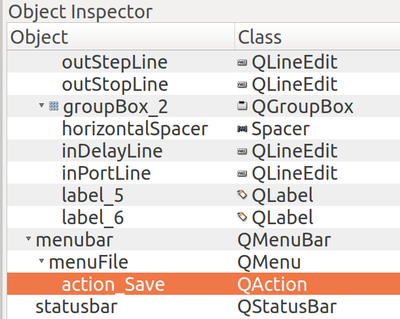
\includegraphics[width=0.6\textwidth]{images/save_menu.png}
\end{center}

If you grabbed the \textbf{scan\_window.ui} from the
\href{https://github.com/PFTL/SimpleDaq/tree/master/PythonForTheLab/View/GUI}{Github
repository} you probably found that there is a menu at the top, called
\mintinline{python}{File} with a \mintinline{python}{Save} option. Having a File menu is the
normal behavior of most programs in most systems, making it an intuitive
place to find such an option. Working with the Menu is almost as easy as
working with a button, you just need to connect the appropriate signal
to the appropriate method in the class. If you open the design file in
the Qt Designer, you will find an element called \mintinline{python}{action_Save}
that appears as a \mintinline{python}{QtAction} instead of a button. Details are not
important, you should just know that inside of menus you will find
actions and not buttons. However, for the purposes of the program, they
work in pretty much the same way. You have to update the
\mintinline{python}{__init__} method to hook the proper signal:

\begin{minted}{python}
self.action_Save.triggered.connect(self.save_data)
\end{minted}

\begin{center}
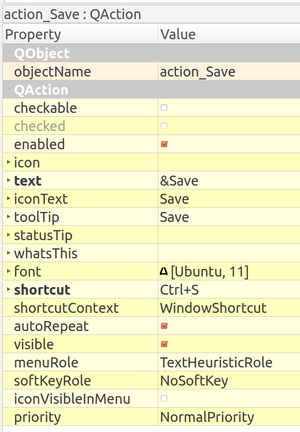
\includegraphics[width=0.6\textwidth]{images/save_shortcut.png}
\end{center}

As easy as that. If you followed the previous exercise, you should have
already defined a method for saving data, so you can just use it. As an
extra, bear in mind two more things. When you define the name for the
menus and the actions you are going to place inside, you can use the
special character \mintinline{python}{&} to make it possible to select that menu by
pressing Alt plus the letter the immediately follows. Therefore, if you
call the menu \mintinline{python}{&File}, when you press Alt+F the menu will be
opened. The same with the action, that is called \mintinline{python}{&Save}.
Therefore, Alt+F opens the File menu, and if you press S it will save
the data. This is handy to go quickly through more complex menus without
using the mouse. You can also define a shortcut for your action, and you
do so directly from within the designer, as is shown in the image.
Whenever you press Ctrl+S you are going to save the data.

Saving data as you have done up to now is handy but lacks some
functionality. For example, you are never asking the user where to save
the data. If you are the only user of your program and you have a folder
where you store all the data, it is a safe bet to default to that
folder. If you are planning to have more users, it is imperative that
you give the users the option to choose. Fortunately, it is incredibly
easy, you can do so with only one line of code:

\begin{minted}{python}
self.directory = str(QtWidgets.QFileDialog.getExistingDirectory(
                    self, "Select Directory", self.directory))
\end{minted}

This will open a dialog where the user can select the directory where to
save the data. For it to work, remember to initialize the variable
\mintinline{python}{self.directory} within the \mintinline{python}{__init__} method. If you
initialize it to an existing directory (for example
\mintinline{python}{C:\textbackslash{}\textbackslash{}Data}), the dialog will start
in that specific place, perhaps saving some searching time to the user.
If not, just initialize it to \mintinline{python}{None} and the dialog will start in
your current directory. Now that you have a directory, don't forget to
use what you have already learned, i.e., don't forget to use
\mintinline{python}{os.path.join}. Also, next time you save data, you will start in
the same directory than last time (\mintinline{python}{self.directory}).

\exercise{Now every time the user wants to save data, a dialog appears asking for
the directory. Find a way to ask for the directory only once and assume
that the next time the file will be saved in the same directory.}

It is also important to be able to add elements to the menu from Python.
Sometimes you are using a designer file that you don't want to modify,
because it is shared amongst different developers, but you still want to
personalize your own program. Following the examples below, you will be
able to create a new menu called \mintinline{python}{Scan}, next to the
\mintinline{python}{File} menu, with two actions, one for starting and one for
stopping a scan. First, you can create a new menu by doing to following:

\begin{minted}{python}
menubar = self.menuBar()
self.scanMenu = menubar.addMenu('&Scan')
\end{minted}

The first line is responsible for addressing the menu bar of the main
window. It follows the same pattern as for when you used the layout of
the central widget. The second line adds a new menu to the menu bar,
called \mintinline{python}{scanMenu} and will display the text \mintinline{python}{Scan}. Again,
the \mintinline{python}{&S} means that you will be able to open the menu by
pressing Alt+S. Next, you have to define the proper actions to add to
the menu:

\begin{minted}{python}
self.start_scan_action = QtWidgets.QAction("Start Scan", self)
self.start_scan_action.setShortcut('Ctrl+Shift+S')
self.start_scan_action.setStatusTip('Start the scan')
self.start_scan_action.triggered.connect(self.start_scan)
\end{minted}

In the first line, you create the action and you set its name to \mintinline{python}{'Start
Scan'}. The \mintinline{python}{self} is to explicitly set the parent for the
action, in your case it is the \mintinline{python}{ScanWindow}. Then you set the
shortcut for the action, in this case, Ctrl+Shift+S. The status tip is
something you haven't use so far, but it will help the user to
understand what will happen if the action is triggered. If you look in
your program, you will see that the message is being displayed at the
bottom of the screen. The last line connects what happens when the
action is triggered, in your case, a scan is started. The only missing
thing is to add the action to the menu, like this:

\begin{minted}{python}
self.scanMenu.addAction(self.start_scan_action)
\end{minted}

\warning{Adding keyboard shortcuts is a great way of shortening both the
development time and the interaction with the interface. It is much
faster pressing Ctrl+S than going with the mouse to the menu, etc.
However, it is important to document every shortcut that you add to your
program. Some are intuitive and the user may try them without thinking,
like the saving. However, imagine that you create a shortcut Alt+S to
start a scan, Alt+F to stop it, etc. You should seriously consider
adding a separate text file to your project describing the
available shortcuts.}

Adding elements to the menu is very handy because it allows you to add a
lot of functionality without cluttering the user interface. Menus can
also be nested, you could have added the scan menu to the file menu, for
example. Now that you are able to start the scan, you should also be
able to stop it.

\exercise{Add a new entry to the menu that allows the user to stop the scan. Pay
attention to the shortcut that you specify.}

For simple programs, you can still work with buttons on the screen. For
more complex programs, you may need to have a clear interface, perhaps
just plotting data and extra options in the menu, that doesn't get in
the way.

\section{Quitting the program}\label{quitting-theprogram}
Your program is very functional, you can acquire and save data, you
check that the user does not trigger more than one scan at a time.
However, there is a very important piece missing. When the user quits
the program, the communication with the device is suddenly interrupted,
which is not the desired behavior. To prevent this, you can add an extra
method for quitting. You only need to overwrite a method inherited from
\mintinline{python}{QMainWindow}:

\begin{minted}{python}
def closeEvent(self, event):
    super().closeEvent(event)
\end{minted}

In this case, nothing is happening because you are just relaying the
method to the parent class' method. However, you can add any code you
want to execute before calling \mintinline{python}{super().closeEvent}. For example,
you could finalize the communication with the device:

\begin{minted}{python}
def closeEvent(self, event):
    print('Closing the window')
    super().closeEvent(event)
\end{minted}

At this point is where you realize that you haven't developed a way of
finishing the communication with the device from the experiment class
nor from the model. However, the driver indeed has a \mintinline{python}{finalize}
method. Suddenly, you realize that you missed an important feature
upstream. You should be aware that in the design pattern that you are
using, from the View you should interact only with the experiment model,
and not directly with the driver. Therefore, to add this new
functionality you need to solve the following exercises in order:

\exercise{Add a method \mintinline{python}{finalize} to the base {DAQ} model.}

\exercise{Reimplement the method \mintinline{python}{finalize} in the \mintinline{python}{AnalogDaq}
model, using the finalize method from the driver.}

\exercise{Create a method in the experiment model that handles what happens when
the experiment is over. For example, communication with the {DAQ}
should be ended with the \mintinline{python}{finalize} method. Perhaps you want to
add something else, such as forcing the save of the parameter metadata
or the data itself.}

\exercise{Update the method \mintinline{python}{closeEvent} in the \mintinline{python}{ScanWindow} in
order to use the finalizing method of your experiment class.}

\section{Conclusions}\label{conclusions}
This is the most rewarding chapter of the book and, alas, the last one.
You have made the jump from a working {GUI} to a usable interface. It is
very important to point out that many of the things you have developed
in this chapter were so easy because of how you structured the different
classes in the previous chapter. For example, the method
\mintinline{python}{do\_scan} in the experiment class was developed in such a way
that it makes it very easy to add and trigger it from the {GUI}.

If you start a project from scratch, you will be tempted to skip some
steps in order to have results faster. Trying to reach your objectives
earlier is very valid, and there are many scenarios where there will be
no further development of your code. In those cases, take the shortcut
and deliver results as fast as you can. However, sometimes you know you
are building something to last. In those cases do not jump ahead. Take
the time you need to reflect on how do you see the future of the code
you are writing. There are going to be different things to polish here
and there, but if the basis is well developed, you are going to save a
lot of time when trying to add new functionalities.

In the case of code that you thought it was never going to grow and
suddenly you start using it very often, don't be afraid of doing a
refactoring and transforming older scripts into classes, modules, etc.
Remember always a general rule of thumb: if you are copy/pasting lines
of code more than twice, then you should have done something
differently. You could have written a function that takes care of your
process, or a class, etc.

In this chapter, you have achieved something that very few people can
say they can do. You have built an interface for a real-world
experiment. You can acquire a signal, change the output, change the
input, change the ranges. You can also save the data and the metadata.
However, there is still much more that can be improved and developed. Of
course, in the real world, once you have a working application, you can
add new options when the need arises or when you have some free time.

\section{Where to go next}\label{where-to-gonext}
At this point, you have acquired a lot of knowledge that you can put
into action. The first logical step is to test what you have learned
from your own experiment. You can go through the steps of the book,
adapting each piece of code to your needs. Don't be afraid of reusing
the pieces of code such as windows and models that can be useful for
your project.

If you are willing to continue expanding the options of the {GUI} that
you have just built, here are some ideas. First, you can build a monitor
for the signal. A monitor is a plot that constantly updates the value
measured, while the x-axis shows the time. You should configure some
parameters, such as the refresh rate, the delay between acquisitions,
and the total time to acquire the signal. You can also create a new
window that holds all the configuration parameters present in the {YAML}
file. For example, the current {GUI} doesn't allow you to change the
current user.

If you are interested in a more fundamental project, you can think about
how to deal with sensors connected to a {DAQ}. There is a common
pattern, in which a voltage is converted into another quantity. For
example, an analog output connected to a piezo stage would transform
voltages into distances. In the example built in this book, you are
measuring a voltage, which can be converted to a current if you know the
resistance connected. Dealing with calibrations, sensors, and actuators
can be achieved through new yaml files and models for the experiment.

Of course, there are many more topics that can be useful for different
researchers. If you have any suggestions, doubts or have found mistakes
please contact us, we are always eager to hear from our readers.
